\section{EUTXO, Informally...}

\begin{frame}{Contract Continuity}
\begin{itemize}
\item New data value on outputs
\item More information available to validators
\item Restrict discussion to state machines here
  \begin{itemize}
  \item However, much more computational patterns are possible
  \item e.g. the entirety of \alert{Marlowe}, a DSL for financial contracts, has
been implemented as a state machine on top of EUTXO.
  \end{itemize}
\end{itemize}
\end{frame}

\begin{frame}{Example: Multi-signature Contract}

\begin{itemize}
\item \textbf{n-out-of-m} signature scheme
\item Plain UTXO requires off-chain communication
\item Can be expressed as a simple state machine:
\end{itemize}

\centering
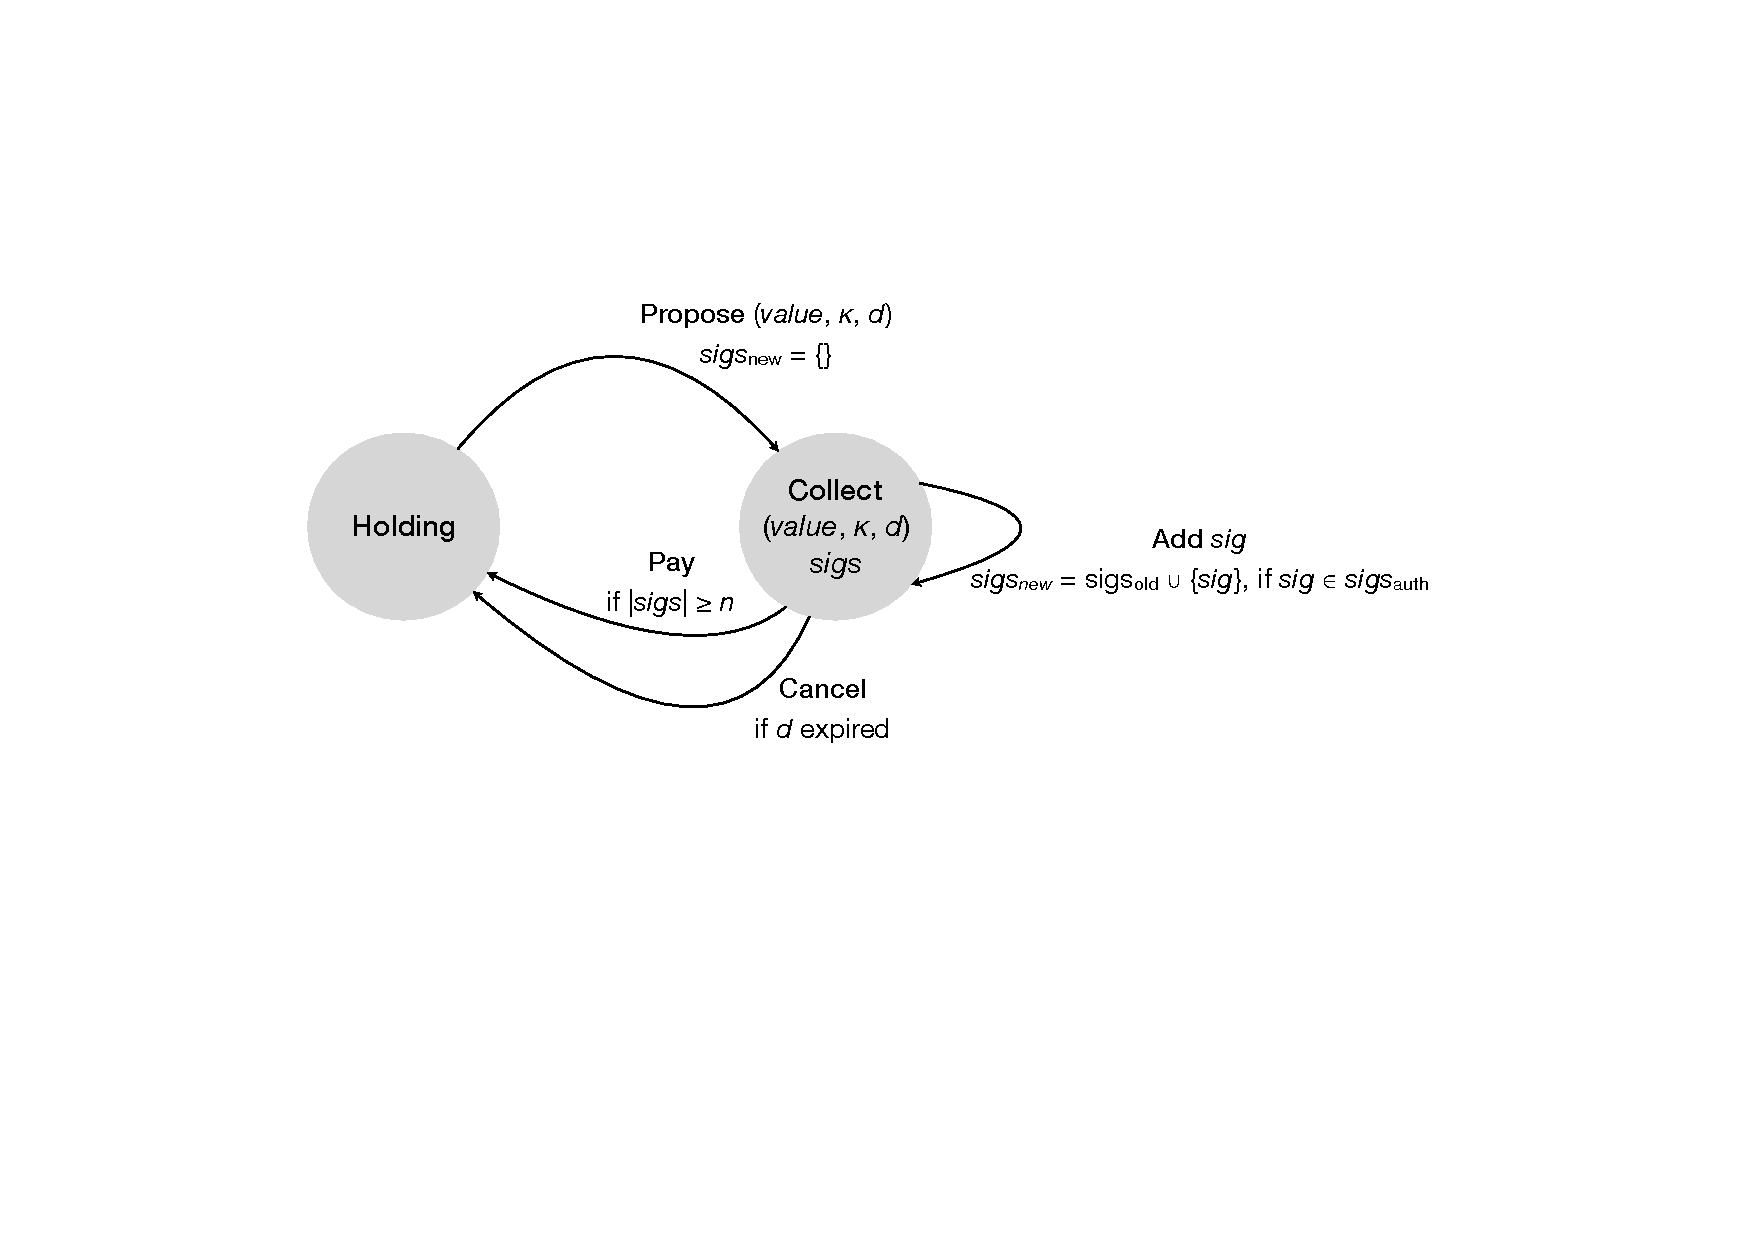
\includegraphics[width=\textwidth]{EUTxO_MultiSig_States.pdf}

\end{frame}

\begin{frame}{Example: Implementation in EUTXO}

\begin{itemize}
\item State machine is associated to a \textit{validator} function
\item \textit{Data values} in outputs correspond to states
  \begin{itemize}
  \item $\in \{ \msf{Holding} , \msf{Collecting} \}$
  \end{itemize}
\item Validator takes one of four possible transitions
  \begin{itemize}
  \item $\in \{ \msf{Propose} , \msf{Add} , \msf{Cancel} , \msf{Pay} \}$
  \item Choice provided by the \textit{redeemer} of the spending input
  \end{itemize}
\end{itemize}

\end{frame}
